\subsection{An approximate calibration to research expenditure}
\label{subsec:rewrite-rsi-research-share}

I now use research expenditure rather than the decline in the AI-service
price to guide the choice of $\chi$. For the United States in 2025,
\citet{korinekmckelvey2026} estimate training compute expenditure of
\$109.58 billion. Relative to nominal GDP of \$30,762.099 billion, this
implies research expenditure of approximately $0.3562\%$ of GDP.\footnote{The
compute estimate is from Table 3 of \citet{korinekmckelvey2026}. Annual
nominal GDP is the BEA series \texttt{GDPA}, available through
\href{https://fred.stlouisfed.org/data/GDPA}{FRED}, accessed September 14, 2026.}
The compute estimate uses rental-equivalent costs and assigns half of total
AI compute spending to training and research. It is a proxy for $M$, not a
direct observation of expenditure on autonomous RSI or of all corporate
R\&D. I use this US ratio as a benchmark without changing the remaining
macroeconomic parameters.

This exercise reports the unit-elastic case, $\sigma=1$. I retain the
fixed-efficiency pre-RSI BGP of Section~\ref{subsec:rewrite-rsi-activation}:
AI is already used in production, $B_0=0.01\overline B$, and initial
capital satisfies $K_0/Y_0=3.30$. These initial conditions preserve the
same production quantities and prices when RSI becomes available
unexpectedly at date zero. Consumption and research adjust endogenously.
Table~\ref{tab:rewrite-research-share-parameters} reports the parameters
and initial stocks.

\begin{rewriteParameterTable}{Lower research expenditure: parameters and initial stocks}{tab:rewrite-research-share-parameters}
$\omega_X$ & 0.10 & AI production weight & Same assumed value as in the preceding exercises; not fitted to industry revenue.\\
$\omega_L$ & 0.90 & Effective-labor weight & Computed as $1-\omega_X$.\\
$\chi$ & 1.4378 & Research productivity after activation & Approximate expenditure calibration at $\sigma=1$: $0.06374\%$ against $0.06638\%$ (2023 US proxy); fixed across elasticities.\\
$\sigma$ & 0.90; 1; 1.10; 1.50 & AI--labor substitution & Same arbitrary scenarios as in the preceding exercises.\\
$\overline B$ & 1,360.992139 & AI-efficiency upper bound & Same $1.10\mathcal B(1.50)$ as before; arbitrary scenario, not estimated.\\
\midrule
$A_0,N_0$ & 1; 1 & Initial technology and population & Same unit normalizations.\\
$B_0$ & 13.609921 & Initial AI efficiency & $0.01\overline B$; same arbitrary initial distance.\\
$K_0$ & 3.433645; 4.649320; 5.036956; 5.504667 & Initial capital, by $\sigma$ & Same fixed-efficiency BGP stocks with existing AI; Equation~\eqref{eq:rewrite-rsi-initial-ratio}.\\
$K_0/Y_0$ & 3.30 & Initial capital--output ratio & Derived from the pre-RSI BGP and preserved at activation.\\
\end{rewriteParameterTable}


I compare the empirical ratio with the model's expenditure and output
integrated over the first year:
\begin{equation}
 \frac{\int_0^1 M_t\,\dd t}{\int_0^1 Y_t\,\dd t}
 \simeq \frac{109.58}{30{,}762.099}=0.00356218.
 \label{eq:rewrite-research-share-target}
\end{equation}
This is an annual expenditure ratio, not the instantaneous $M_0/Y_0$.
On the numerical branch examined, the annual ratio reaches a local maximum
near $\chi=81.084809$. I retain this value as an approximate calibration:
the model produces $0.3215\%$, or $9.75\%$ less than the empirical proxy.
The discrepancy is reported rather than absorbed into numerical tolerances;
the equilibrium checks remain unchanged. Appendix~\ref{app:rewrite-algorithm}
documents the search, verification and replication files.

The resulting transition remains rapid. The AI-service price falls by
$90.6\%$ over 27 months, although no price decline is targeted. Research
expenditure is initially $0.4521\%$ of output, but its annual ratio falls
from $0.3215\%$ in the first year to $0.2114\%$ in the second. Matching a
high expenditure level approximately therefore does not also match the
recent growth of research expenditure or produce a gradual RSI activation.
Output per person and the real wage initially grow at an instantaneous
annual rate of $25.86\%$, not a realized first-year growth rate. Their
growth eventually returns to $\gamma=1\%$, and the interest rate returns
to $\rho+\gamma=5\%$.

Figures~\ref{fig:rewrite-research-share-accumulation}--\ref{fig:rewrite-research-share-distribution}
retain the earlier panels and time windows, with one equilibrium path in
each panel. At unit elasticity, labor's income share remains $60.3\%$
throughout the transition, and AI revenue remains $6.7\%$ of output.
Research changes the division of that revenue between expenditure and
net profit, not the factor shares. The initial size of the AI industry
is not fitted in this exercise.

\begin{figure}[H]
 \centering
 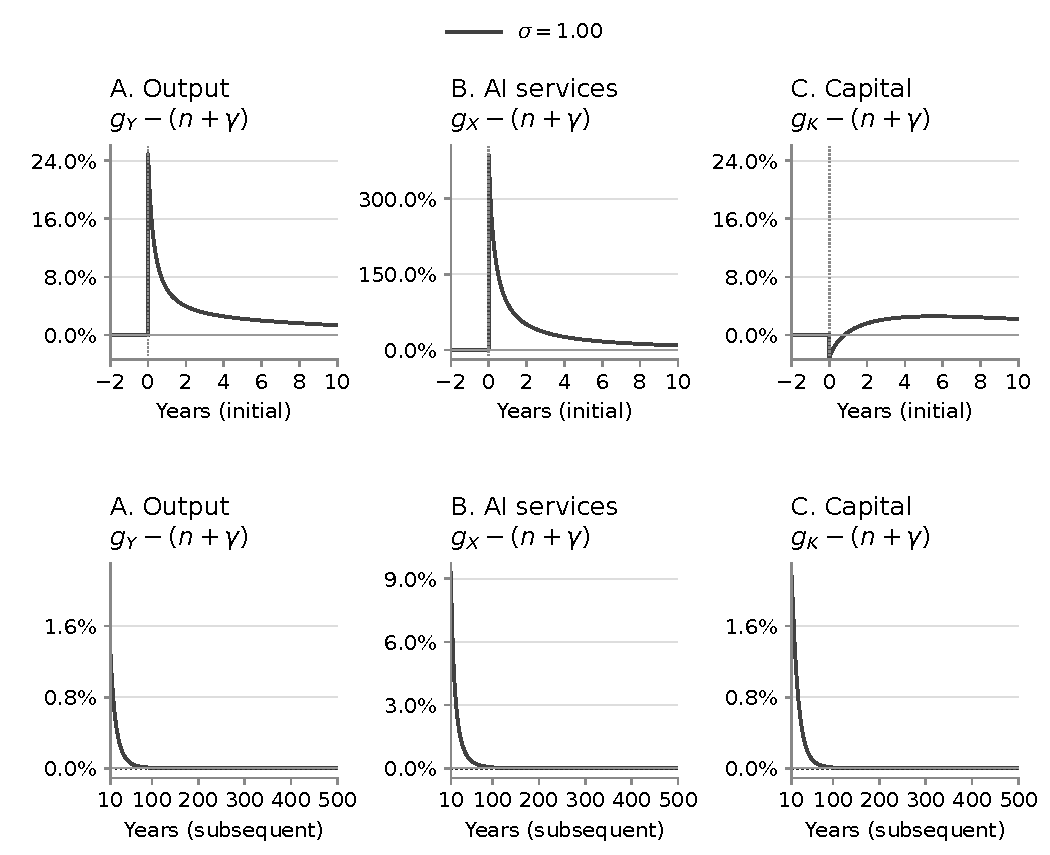
\includegraphics[width=\textwidth]{figures_rewrite/equilibrium_rsi_research_share_approximate_unit_accumulation_growth_windows.pdf}
 \caption{Research-expenditure calibration at $\sigma=1$: growth of output,
 AI production services and capital per unit of effective labor. Rates are
 instantaneous annual rates. The upper row shows years $-2$ to 10 and the
 lower row years 10--500. Vertical scales differ between rows; output and
 capital share a scale within each row. The vertical line marks RSI
 activation, and dotted horizontal lines mark the unit-elastic limits.}
 \label{fig:rewrite-research-share-accumulation}
\end{figure}

\begin{figure}[H]
 \centering
 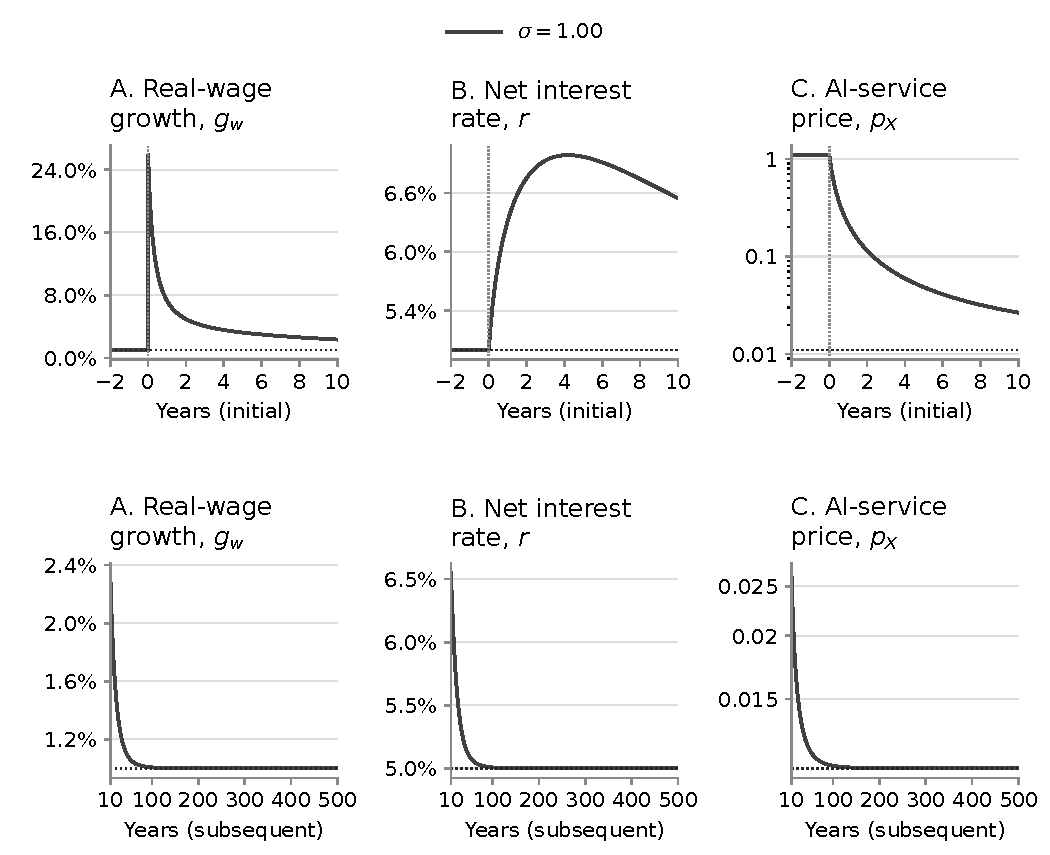
\includegraphics[width=\textwidth]{figures_rewrite/equilibrium_rsi_research_share_approximate_unit_growth_returns_windows.pdf}
 \caption{Research-expenditure calibration at $\sigma=1$: real-wage
 growth, the net interest rate and the AI-service price. The price is in
 final-good units on a logarithmic scale and is not a calibration target.
 Vertical scales differ between the initial and subsequent windows.
 Dotted horizontal lines mark the unit-elastic limits.}
 \label{fig:rewrite-research-share-prices}
\end{figure}

\begin{figure}[H]
 \centering
 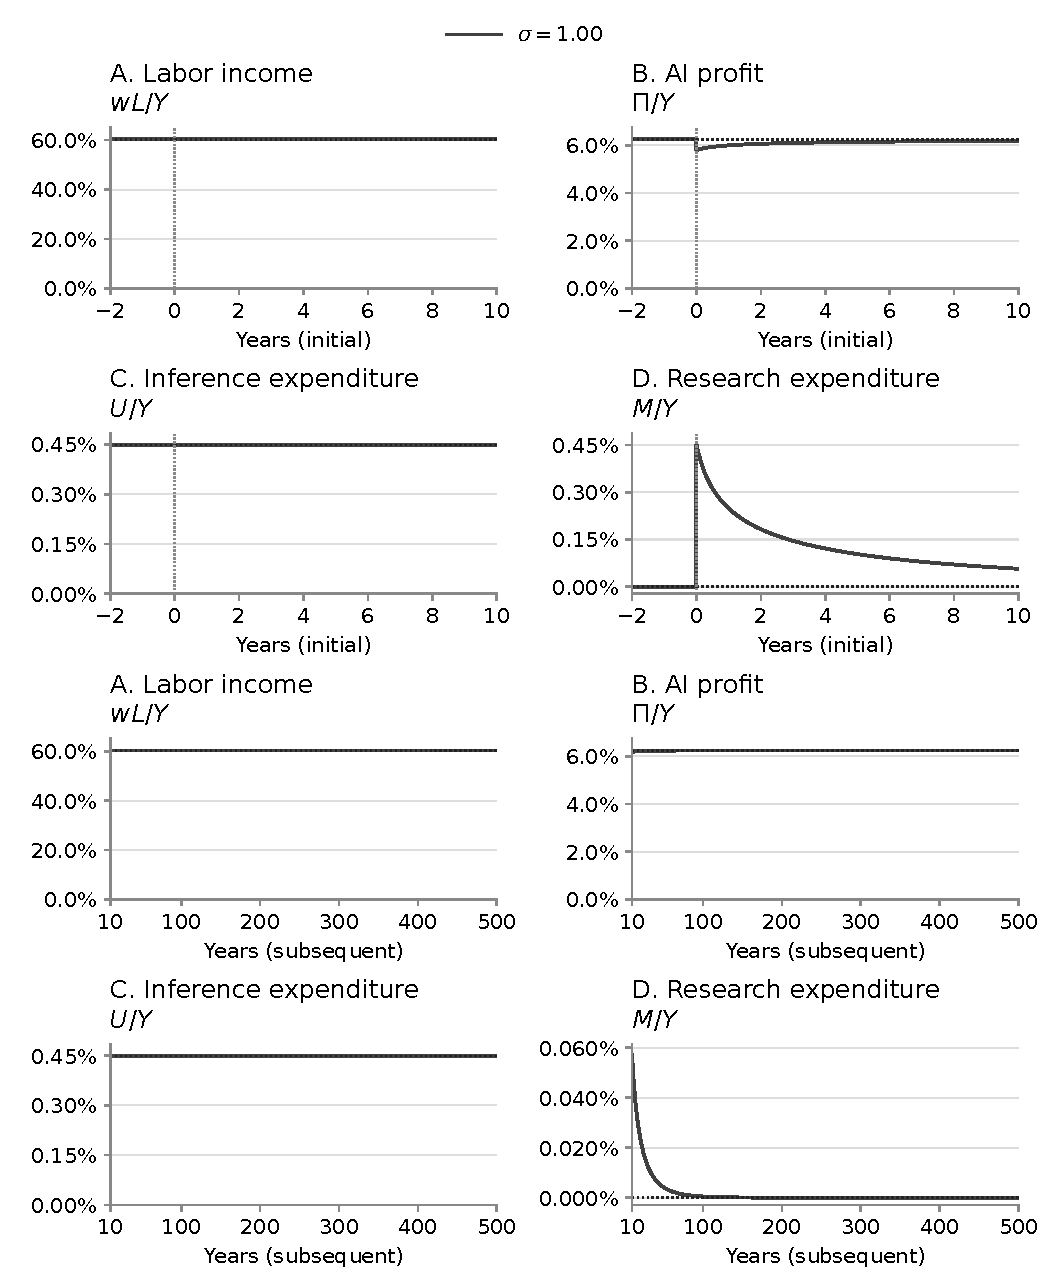
\includegraphics[width=\textwidth]{figures_rewrite/equilibrium_rsi_research_share_approximate_unit_ai_distribution_windows.pdf}
 \caption{Research-expenditure calibration at $\sigma=1$: labor income,
 AI net profit, inference expenditure and research expenditure as shares
 of output. The first two rows show years $-2$ to 10 and the last two show
 years 10--500. The instantaneous research share differs from the annual
 ratio in Equation~\eqref{eq:rewrite-research-share-target}. Dotted horizontal
 lines mark the unit-elastic limits; the gross capital share remains $0.33$.}
 \label{fig:rewrite-research-share-distribution}
\end{figure}
